\chapter{Applications when you have networks}
\label{sec:ch8}

In this section, we'll proceed much the same as the preceding section. We'll learn how to learn from networks, but particularly in the case where you have two networks. When you have two networks, there are some nuances to analytical procedures that arise, and many special questions that you can ask between the two networks. 

In particular, when we have two networks, we can start to make explicit comparisons across networks assuming they are sufficiently similar. In general, this means that we will assume that the networks that we are comparing have the same nodes, and that the edges are the only things that (might) differ across them. In this case, we can learn properties about network models, and make comparisons between the networks by studying how similar (or different) these properties are between the networks. When the networks are not sufficiently similar, in that their node sets are not necessarily the same, we will finish the chapter off by discussing strategies to align (or, \textit{match}) the nodes to make the node sets near equivalent between the networks. 

\section{Two-sample testing for networks}
\paragraph*{Co-authored with Sambit Panda}
\label{sec:ch8:twosample}

In Section \ref{sec:ch6:multinet}, we learned several techniques for dealing with multiple networks. When you find networks in your data, a fundamental question that you might have is how to determine whether the networks differ. This problem is another instance of a two-sample test, much like the two-sample test that we learned about in Section \ref{sec:ch7:testing:twosample}. Remember that a \textit{two-sample test} was a test to determine whether two samples of data were different. 

To do this, we'll return to the alien and human brain networks example, from Case Study \ref{box:ch6:multinet:ex}. There are $n=100$ brain areas, which represent the nodes of the network. This time, we find a third group of aliens, and their brain structure is much more similar to humans than our original group of aliens (they are still homophilic). However, this group of aliens tends to have heterogeneities in the node degrees: nodes with lower indices have a higher degree than nodes with higher indices, whereas the human brains tend to have more homogeneous structurings.

Let's imagine that we have one human brain, and one alien brain:

\begin{lstlisting}[style=python]
from graspologic.simulations import sbm
import numpy as np
from graphbook_code import dcsbm, generate_dcsbm_pmtx, \
                           generate_sbm_pmtx

n = 100  # the number of nodes
M = 8  # the total number of networks
# human brains have homophilic block structure
Bhum = np.array([[0.2, 0.02], [0.02, 0.2]])
# alien brains add degree-correction
theta_alien = np.tile(np.linspace(1.7, 0.3, 50), 2)

# generate 4 human and alien brain networks
A_human, z = sbm([n // 2, n // 2], Bhum, return_labels=True)
A_alien = dcsbm(z, theta_alien, Bhum)

Phum = generate_sbm_pmtx(z, Bhum)
Palien = generate_dcsbm_pmtx(z, theta_alien, Bhum)
\end{lstlisting}

Plots of the networks are shown in Figure \ref{fig:ch8:twosample:ex}, where their underlying probability matrices are shown in \textbf{(A)} and \textbf{(C)}. Note that the degree-correction factor for the alien brain network has led to the nodes with lower indices in each community to have higher probabilities of being connected to other nodes. Samples of the human and alien brain networks are \textbf{(B)} and the alien brain network in \textbf{(D)}. It is a little bit less obvious that the networks are different when we look at the network samples. 

Just like when we were flipping coins we could not immediately conclude that two coins were different just because they produced a different number of heads in a given number of flips, it would be unwise to conclude that the networks differ fundamentally (they have different probability matrices) just because the samples look different. 

\begin{figure}[h]
    \centering
    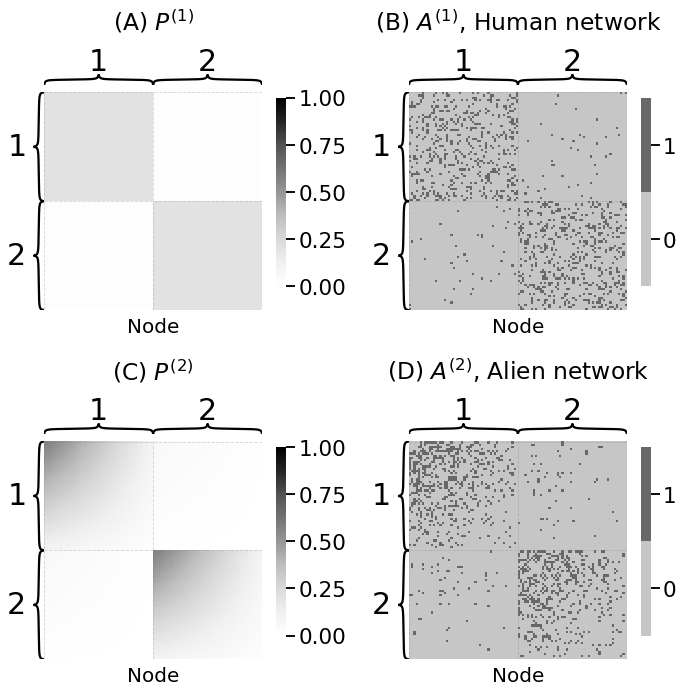
\includegraphics[width=0.7\linewidth]{applications/ch8/Images/ts_ex.png}
    \caption[Human and alien brains]{\textbf{(A)} probability matrix underlying human brain network, \textbf{(B)} brain network from human, \textbf{(C)} probability matrix underlying alien brain network, \textbf{(D)} brain network from alien.}
    \label{fig:ch8:twosample:ex}
\end{figure}

For this reason, it is important for us to build out our two-sample testing procedures, so that we can determine whether the networks differ.

\subsection{Two-sample tests and random networks}

In this section, we'll go a slightly different direction from the last time we saw two-sample testing. When we have two random networks $\mathbf A^{(1)}$ and $\mathbf A^{(2)}$, our first thing that we need to do is determine appropriate models for our networks. If we make the assumption that these networks are $IER_n\left(P^{(m)}\right)$ random networks from Section \ref{sec:ch5:ier}, which are the broadest class of independent-edge random network models, remember that the probability matrix encodes the differences between the two random networks. Therefore, our question is:
\begin{align*}
    H_0 : P^{(1)} = P^{(2)} \text{ against }H_A : P^{(1)} \neq P^{(2)}, \numberthis \label{eqn:ch8:twosample:2shypo_prob}
\end{align*}
or that the edge probability matrices are the same (under the null hypothesis) against that the edge probability matrices differ (under the alternative hypothesis). This is exactly the same question that we would ask about determining whether two coins are different, but generalized to $n \times n$ probability matrices.

Remember, however, that the $IER_n\left(P^{(m)}\right)$ random networks are difficult to deal with (directly) when you only have a single network sample. This means that testing the hypotheses in Equation \eqref{eqn:ch8:twosample:2shypo_prob} is fairly impractical when you only have two networks, because you only have one sample $a_{ij}^{(m)}$ to base your estimate of $p_{ij}^{(m)}$ on. 

\subsection{Latent positition testing}
\label{sec:ch8:twosample:lpt}
For this reason, it is fairly typical to make further assumptions about the network structure. As you learned in Section \ref{sec:ch6:ase}, a typical assumption that we can make is that the networks are $RDPG_n\left(X^{(m)}\right)$ random networks, with latent position matrices $X^{(m)}$. Remember that your latent position matrix $X^{(m)}$ fully describes the probability matrix $P^{(m)}$, so it would be (almost) equivalent to just compare the latent positions directly:
\begin{align*}
    H_0 : X^{(1)} = X^{(2)} \text{ against }H_A : X^{(1)} \neq X^{(2)}, \numberthis \label{eqn:ch8:twosample:2shypo_lpm:dumb}
\end{align*}
or would it? Remember that for a network with a latent position matrix $X^{(m)}$, that for any $d \times d$ rotation matrix $W$, by the non-identifiability problem in Section \ref{sec:ch6:spectral:nonidentifiable}:
\begin{align*}
    P^{(m)} &= X^{(m)}X^{(m)}^\top = X^{(m)}WW^\top X^{(m)}^\top
\end{align*}
This means that even if $P^{(1)}$ and $P^{(2)}$ were identical, we could define their latent position matrices differently, and still end up with the same random network, by having $X^{(2)} = X^{(1)}W$ for some rotation matrix $W$. For this reason, we'll make our hypothesis ``robust'' to this challenge, and test:
\begin{align*}
    H_0 :& X^{(1)} = WX^{(2)}\text{ for some rotation matrix $W$} \\
    H_A :& X^{(1)} \neq WX^{(2)} \text{ for any rotation matrix $W$}. \numberthis \label{eqn:ch8:twosample:2shypo_lpm:smart}
\end{align*}
In words, our null hypothesis is that the latent positions are identical up to a rotation (for some possible rotation matrix), and our alternative hypothesis is that the latent positions are not rotations of one another (for any possible rotation matrix). 

\subsubsection*{Learning rotations from the data}

From Section \ref{sec:ch6:ase}, we know that we can obtain estimates of $X^{(m)}$ by using the \texttt{ase}, where $\hat X^{(m)} = \texttt{ase}\left(A^{(m)}\right)$. How do we account for the potential that $X^{(1)}$ and $X^{(2)}$ are rotations of one another?

\paragraph*{The orthogonal Procrustes problem}

To estimate a possible rotation, we will need to set up an optimization problem. Our goal is to find the best possible rotation of $X^{(2)}$ onto $X^{(1)}$. 

\begin{floatingbox}[h]\caption{Concept: The Frobenius norm}
\label{box:ch7:twosample:frobnorm}
The Frobenius norm can be thought of as a generalization of the Euclidean norm from Concept \ref{def:ch6:se:eucl_dist} to matrices. If $A$ is a $n \times m$ matrix with entries $a_{ij}$, the Frobenius norm is:
\begin{align*}
    \|A\|_F &= \sqrt{\sum_{i = 1}^n \sum_{j = 1}^m a_{ij}}
\end{align*}
We can use the Frobenius norm to define a distance. If $A$ and $B$ are two matrices with the same number of rows ($n$) and columns ($m$), their Frobenius distance is:
\begin{align*}
    \|A - B\|_F &= \sqrt{\sum_{i = 1}^n \sum_{j = 1}^m (a_{ij} - b_{ij})^2}
\end{align*}
\end{floatingbox}

Using Concept \ref{box:ch7:twosample:frobnorm}, we can define what we mean by the ``best'' possible rotation: the rotation where the Frobenius distance between $X^{(1)}$ and $X^{(2)}$ are minimized. We can describe our goal as:
\begin{align*}
    \text{find }W \text{ where } \left\|X^{(1)} - X^{(2)}W\right\|_F\text{ is minimized}.
\end{align*}
We can equivalently write this goal as:
\begin{align*}
    \hat W &= \text{argmin}_W \left\|X^{(1)} - X^{(2)}W\right\|_F.\numberthis \label{eqn:ch8:twosample:opp}
\end{align*}
The idea is that if $X^{(1)}$ and $X^{(2)}$ are rotations of one another, we can (at least, in theory) for the $d \times d$ rotation matrix $\hat W$ that properly aligns them. If such a rotation exists, the function that we are minimizing $\left\|X^{(1)} - X^{(2)}\hat W\right\|_F$ will have a value of $0$ when we find the correct rotation (because the matrices will be identical). The problem of solving for optimal rotations in Equation \eqref{eqn:ch8:twosample:opp} is known as the \textit{orthogonal Procrustes problem}.

In practice, we only have estimates $\hat X^{(1)}$ and $\hat X^{(2)}$, so we will not find the perfect rotation of $\hat X^{(1)}$ onto $\hat X^{(2)}$ (even if such a rotation exists for $X^{(1)}$ and $X^{(2)}$). Therefore, when we minimize $\left\|\hat X^{(1)} - \hat X^{(2)}W\right\|_F$, we will just want the $\hat W$ that makes them the most similar (in terms of the Frobenius distance). If $X^{(1)}$ and $X^{(2)}$ are the same, we would expect that $\left\|\hat X^{(1)} - \hat X^{(2)}\hat W\right\|_F$ would therefore take a relatively small value.

Programatically, we can code this up as:

\begin{lstlisting}[style=python]
from scipy.linalg import orthogonal_procrustes
from graspologic.models import RDPGEstimator
import numpy as np

d = 2
# estimate latent positions for alien and human networks
Xhat_human = RDPGEstimator(n_components=d).fit(A_human).latent_
Xhat_alien = RDPGEstimator(n_components=d).fit(A_alien).latent_
# estimate best possible rotation of Xhat_alien to Xhat_human by 
# solving orthogonal procrustes problem
W = orthogonal_procrustes(Xhat_alien, Xhat_human)[0]
observed_norm = np.linalg.norm(Xhat_human - Xhat_alien @ W, ord="fro")
\end{lstlisting}

This gives us the value shown in Figure \ref{fig:ch8:twosample:lpt}(A), in gray. A relatively small value, relative what exactly?

\begin{figure}
    \centering
    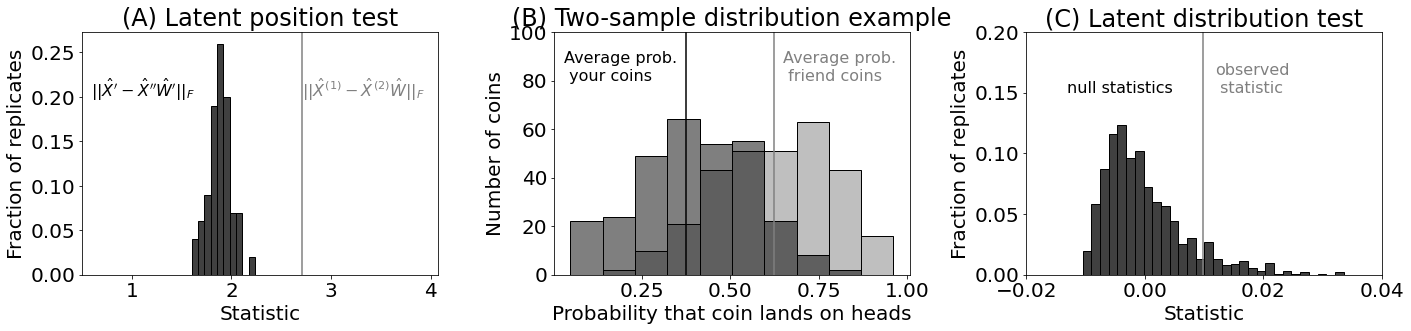
\includegraphics[width=\linewidth]{applications/ch8/Images/ts_ldt_ex.png}
    \caption[Latent position and latent distribution testing]{\textbf{(A)} The observed statistic from the data (gray) compared to a histogram from the $r=100$ parametric replicates (black). \textbf{(B)} A comparison of two buckets of coins, where each coin has a different probability of landing on heads. \textbf{(C)} The observed statistic from the data (gray) compared to a histogram from the $r=1000$ replicates (black).}
    \label{fig:ch8:twosample:lpt}
\end{figure}

\subsubsection{Generating a null distribution through parametric bootstrapping}

If you recall from Section \ref{sec:ch7:testing:twosample}, we learn with hypothesis tests by looking at how well the data reflect the null hypothesis; that is, that the estimated latent positions (computed from the data) are identical (up to a rotation). 

When you have estimates computed from the data, ideally, you will be able to determine directly (by the nature of the data and the assumptions that you make) exactly how ``anomalous'' the difference that you observe is relative what you would expect under the null hypothesis. In the case of the contingency tables from Section \ref{sec:ch7:testing:twosample}, the Fisher's exact test used the assumptions that we made (that the two samples were independent binary events) to compute how ``anomalous'' the contingency table that we observed was. 

In this case, however, without more assumptions we can't quite compute this value exactly. In the interest of keeping assumptions to a minimum, a popular strategy is to use what is known as a \textit{bootstrap}. A \textit{bootstrap} is a technique which attempts to quantify the sampling distribution of some quantity (a \textit{statistic}) that is computed from the data. The \textit{sampling distribution} refers to the distribution of the statistic $\left\|\hat X^{(1)} - \hat X^{(2)}\hat W\right\|_F$, where $\hat X^{(1)}$, $\hat X^{(2)}$, and $\hat W$ are computed from the data.

The way that we will do this is that we will use the parameter $\hat X^{(1)}$ as the latent position matrix for two new random networks, $\mathbf A'$ and $\mathbf A''$. These two random networks have an identical latent position matrix: $\hat X^{(1)}$. Then, we will generate two new samples of these random networks with the same latent position matrix:

\begin{lstlisting}[style=python]
from graspologic.simulations import rdpg

def generate_synthetic_networks(X):
    """
    A function which generates two synthetic networks with
    same latent position matrix X.
    """
    A1 = rdpg(X, directed=False, loops=False)
    A2 = rdpg(X, directed=False, loops=False)
    return A1, A2

Ap, App = generate_synthetic_networks(Xhat_human)
\end{lstlisting}

We then use these two new networks, and again estimate latent position matrices for these:

\begin{lstlisting}[style=python]
def compute_latent(A, d):
    """
    A function which returns the latent position estimate
    for an adjacency matrix A.
    """
    return RDPGEstimator(n_components=d).fit(A).latent_

Xhat_p = compute_latent(Ap, d)
Xhat_pp = compute_latent(App, d)
\end{lstlisting}

Finally, just like we aligned $\hat X^{(1)}$ and $\hat X^{(2)}$ via the ``optimal rotation'' $\hat W$, we will align $\hat X'$ and $\hat X''$ via the ``optimal rotation'' $\hat W'$. Then, we recompute our statistic of interest $\left\|\hat X' - \hat X''W'\right\|_F$ using these new samples, where the underlying latent positions were truly identical:

\begin{lstlisting}[style=python]
def compute_norm_orth_proc(A, B):
    """
    A function which finds the best rotation of B onto A,
    and then computes and returns the norm.
    """
    R = orthogonal_procrustes(A, B)[0]
    return np.linalg.norm(A - B @ R)

norm_null = compute_norm_orth_proc(Xhat_p, Xhat_pp)
\end{lstlisting}


We keep repeating this process again and again, and over time, we gradually get some idea of what $\left\|\hat X^{(1)} - \hat X^{(2)}\hat W\right\|_F$ would look like if the true latent positions $X^{(1)}$ and $X^{(2)}$ were identical up to a rotation $W$. This is known as a \textit{parametric bootstrap}. It is called \textit{parametric} because we are using the assumption that the networks are RDPGs to generate what $\hat X^{(1)}$ and $\hat X^{(2)}$ would look like under the null hypothesis (that they are identical up to a rotation). 

The statistics that we compute from the parametric null replicates (the statistics under the null hypothesis) are indicated by the histogram on Figure \ref{fig:ch8:twosample:lpt}(A), in black. Notice that the statistic is less extreme than the one that we observed from the data, shown in gray. 

The below code will repeat this procedure $r=100$ times (the number of \textit{replicates} of the bootstrap resampling), and keep track of the computed statistics under the null hypothesis:

\begin{lstlisting}[style=python]
def parametric_resample(A1, A2, d, nreps=100):
    """
    A function to generate samples of the null distribution under H0
    using parametric resampling.
    """
    null_norms = np.zeros(nreps)
    Xhat1 = compute_latent(A1, d)
    for i in range(0, nreps):
        Ap, App = generate_synthetic_networks(Xhat1)
        Xhat_p = compute_latent(Ap, d)
        Xhat_pp = compute_latent(App, d)
        null_norms[i] = compute_norm_orth_proc(Xhat_p, Xhat_pp)
    return null_norms

nreps = 100
null_norms = parametric_resample(A_alien, A_human, 2, nreps=nreps)
\end{lstlisting}

What we see is that $||\hat X^{(p)} - \hat X^{(r)}\hat W||_{F}$ is much larger than the almost all of the values of $|| \hat X' - \hat X''\hat W'||_{F}$ that we calculated. We will use this to estimate a $p$-value, and we will say that the $p$-value of $H_0$ against $H_A$ is the fraction of times that when the underlying latent positions were equal (for each replicate of our parametric bootstrap), the value of the statistic that we calculated from the observed data exceeded the statistic that we calculated from the replicate. We add one to the numerator and denominator, since we observed one instance of a value at least as big as that in the observed data: the observed data itself. 

This means our $p$-value is:

\begin{lstlisting}[style=python]
pval = ((null_norms >= observed_norm).sum() + 1)/(nreps + 1)
print("estimate of p-value: {:.3f}".format(pval))
# estimate of p-value: 0.010
\end{lstlisting}

We then repeat this process, but we use $A^{(2)}$ as our reference point instead of $A^{(1)}$. The overall $p$-value is the maximum of the two $p$-values produced with this procedure.

This is called the \textit{latent position test}, and it is implemented directly by \texttt{graspologic}. Note that the $p$-value that you obtain from this process might differ every time you run the test, since there is randomness in your generation process of the $A'$s and the $A''$s for every time you repeated the comparison. Making the number of repetitions larger by setting \texttt{n\_bootstraps} to a higher value will tend to yield more stable $p$-value estimates for when we estimate $p$-values using resampling techniques:
\begin{lstlisting}[style=python]
from graspologic.inference import latent_position_test

nreps = 50 # the number of null replicates
lpt = latent_position_test(A_human, A_alien, n_bootstraps = nreps, n_components=d, workers=-1)
print("estimate of p-value: {:.5f}".format(lpt[1]))
# estimate of p-value: 0.00100
\end{lstlisting}
The $p$-value is low, and below a typical decision threshold of $\alpha = 0.05$. This means we have evidence to reject the null hypothesis in favor of the alternative: the latent position matrix for a human brain network differs from the latent position matrix for an alien brain network (by more than just a rotation).

Next, let's see what happens if we have two networks with the same underlying latent position matrices. We'll make a second network from a human, and use the latent position test to determine whether the networks have identical latent position matrices (up to a rotation):
\begin{lstlisting}[style=python]
# generate a new human brain network with same block matrix
A_human2 = sbm([n // 2, n // 2], Bhum)

lpt_hum2hum = latent_position_test(A_human, A_human2, n_bootstraps=nreps, n_components=d, workers=-1)
print("estimate of p-value: {:.5f}".format(lpt_hum2hum[1]))
# estimate of p-value: 0.65347
\end{lstlisting}
The $p$-value is relatively large, so with $\alpha = 0.05$, we fail to be able to reject the null hypothesis. We conclude that our data does not support that our two human networks have different underlying latent position matrices (which is great, because they are the same). The latent position test is described in \cite{Tang2017Apr}.

\subsection{Latent distribution testing}

To motivate a latent distribution test, we're going to return to yet another coin example. Imagine that you and a friend do not each have a single coin like the examples that you have seen so far, but you each have a container of $300$ coins. Each of these $300$ coins can be identified as the coin $\mathbf x_i^{(y)}$ or $\mathbf x_i^{(f)}$, your $i^{th}$ coin or your friend's $i^{th}$ coin. 

The outcomes $\mathbf x_i^{(y)}$ and $\mathbf x_i^{(f)}$ are random. These coins all have different probabilities of landing on heads, $\mathbf p_i^{(y)}$ and $\mathbf p_i^{(f)}$, again for your coin and your friend's coin, respectively, and the probabilities that the *coins* land on heads is random too! Let's say, for sake of example, that your coins have probabilities of landing on heads that tend to be right around $\frac{3}{8}$, but your friend's coins have probabilities of landing on heads right around $\frac{5}{8}$:

\begin{lstlisting}[style=python]
ncoins = 300  # the number of coins in each container

# the probabilities of your coins landing on heads
piy = np.random.beta(a=3, b=5, size=ncoins)

# the probabilities of your friend's coins of landing on heads
pif = np.random.beta(a=5, b=3, size=ncoins)
\end{lstlisting}
You each grab a single coin at random from your containers, and flip them and observe whether they land on heads or tails, the outcomes $x_i^{(y)}$ and $y_i^{(f)}$, respectively. Since the probabilities each coin lands on heads is random here, we can't actually compare the probabilities. But what we can compare are characteristics about your coins' and your friend's coins' probabilities. 

You could ask, for instance, whether the average probability that your coins land on heads is less than the average probability that your friend's coins land on heads. The difference is that we are asking about parameters that underly the random probabilities of the random coins in the experiment, and not about the random probabilities themselves.

Much the same, we could assume that not only are the latent positions for humans and aliens different, but these might be random too, just like the probabilities of the coins in the example you just learned about. What we mean when we say that the latent position matrices are random, we mean that the latent positions for each node, the vectors $\vec x_i^{(1)}$ and $\vec x_i^{(2)}$ for each of the $n$ total nodes, are not necessarily fixed quantities. There might be random variables that underly these too: $\mathbf{\vec x}_i^{(1)}$ and $\mathbf{\vec x}_i^{(2)}$. 

We won't need to go too in-depth here, but the basic idea is that the latent position vectors for each node, $\mathbf{\vec x}_i^{(1)}$ and $\mathbf{\vec x}_i^{(2)}$, have underlying parameters as well, just like the random probabilities for your coins and your friend's coins tended to be around $\frac{3}{8}$ and $\frac{5}{8}$ respectively. All of the characteristics that determine how the human or alien latent position vectors can be realized are governed by functions called the distributions of the latent position vectors. We use the symbol $F^{(1)}$ and $F^{(2)}$, respectively, to denote the distribution of the humans' latent position vectors and the aliens' latent position vectors, respectively. When we ask questions about whether $\mathbf P^{(1)}$ and $\mathbf P^{(2)}$ differ, now our question no longer boils down to just checking whether the latent positions themselves are different, but whether the distributions of the latent positions are different.

did before, we will make null and alternative hypotheses for these situations. Your null hypothesis is going to be that $H_0 : F^{(1)} = F^{(2)}W$, which means that the distributions of the latent positions are the same (like before, we allow for a possible $W$). The alternative hypothesis is going to be that the latent positions for the Moors and the Moops have a different distribution for any possible rotation, $H_A : F^{(1)} \neq F^{(2)}W$.

The general idea is that we will assume as little as possible about the distributions for the latent positions. Two good ways to do this are using an approach called distance correlation \cite{Szekely2007Dec} or multiscale generalized correlation (MGC) \cite{Vogelstein2019Jan}. You can do these very easily using \texttt{graspologic}, through the \texttt{latent\_distribution\_test} function:

\begin{lstlisting}[style=python]
from graspologic.inference import latent_distribution_test

nreps = 50
approach = 'dcorr'  # the strategy for the latent distribution test
ldt_dcorr = latent_distribution_test(A_hum, A_alien, test=approach, metric="euclidean", n_bootstraps=nreps, workers=-1)
\end{lstlisting}

The relevant things to look at for the latent distribution is again the $p$-value:

\begin{lstlisting}[style=python]
print("p-value of H0 against HA: {:.4f}".format(ldt_dcorr[1]))
\end{lstlisting}

The null replicates against the observed test statistic are shown in Figure \ref{fig:ch8:twosample:lpt}(C). For more details on this approach, check out \cite{Alyakin2020}.

\subsection{When would you use the latent distribution test versus the latent position test?}
\label{sec:ch8:twosample:lpt_vs_ldt}

The latent distribution test is called non-parametric because it does not make the assumption that the networks are RDPGs with fixed latent position matrices like we did in the latent position test. In this sense, the latent distribution test tends to be a little bit more general than the latent position test, and will tend to be more \textit{conservative}. In statistics, a \textit{conservative} test is a testing procedure which tends to err on the side of caution: the $p$-values, and consequently your conclusions, will generally tend to err towards shying away from rejecting the null hypothesis. When we obtain results in favor of $H_A$ with conservative tests (such as a small $p$-value), we tend to have a little bit more confidence that our results hold up to scrutiny, which is a good thing if you are trying to convince people you are correct and that your assumptions did not dictate your conclusions.

Moreover, the latent position test assumes that the two networks have node matching: node $1$ in the first network has the same interpretation as node $1$ in the second network, and so on for all $n$ nodes in the network. The latent distribution test does not make this rather limiting assumption: you can perform a latent distribution test when the nodes differ in both interpretation (nodes don't need to be matched) or in number (you could compare networks without the same number of nodes entirely). This makes the latent distribution test a bit more flexible, in general, than the latent position test.

\paragraph*{Generalizing to other network models}

The results that we learned in this section generalize directly to any random network models that can be described as $RDPG_n(X)$ random networks: this includes any network model where the probability matrix has a positive semi-definite structure. As you learned in Section \ref{sec:ch5:psd_block}, this includes many other network models, such as DCSBMs and RDPGs with positive semi-definite block matrices. 

The utility of these techniques, however, likely generalizes beyond just the $RDPG_n(X)$ random networks, and probably includes gRDPG random networks, too. This is because the primary piece of information that is needed to motivate the techniques described here was that $\hat X^{(1)}$ and $\hat X^{(2)}$ were reasonable (unbiased and consistent) estimates of the latent position matrices $X^{(1)}$ and $X^{(2)}$ (up to a rotation). As you learned in Section \ref{sec:ch6:ase:whyuse}, spectral embedding techniques can produce similarly reasonable estimates of latent position matrices for gRDPG random networks too. While there is no direct theory that asserts that the latent position and latent distribution tests are appropriate for gRDPGs, it is pretty reasonable to expect them to apply in for gRDPGs (with potentially non positive semi-definite probability matrices) too. For the latent position test, a key modification would be that the parametric bootstrap would need to consider samples from gRDPG random networks, and not $RDPG_n(X)$ random networks (with the rest of the logic applying as-is).

\subsection{Read on for more information}

Appendix \ref{app:ch12:rdpg} discusses the foundational assumptions for the latent distribution test, the \textit{a posteriori} Random Dot Product Graph. Appendix \ref{app:ch13:spectral} discusses the implications of latent distribution testing with respect to spectral embeddings.

\newpage
\section{Two-sample testing for SBMs}
\label{sec:ch8:twosamplesbm}

In Section \ref{sec:ch8:twosample}, we saw a situation where we had two networks which we thought could be effectively characterized with RDPG. Further, we knew that the communities were the same across both networks: that is, we knew that community $1$ in the first network was the same as community $1$ in the second network, so on and so forth all the way up to community $K$. In this situation, we found that we could test whether the latent positions for the underlying RDPGs are the same; that is, whether $H_0: X^{(1)} = X^{(2)}W$ against $H_A: H^{(1)} \neq X^{(2)}W$. We called this the two-sample hypothesis test for RDPGs. 

What if we can take this a step further, however, and we can say that the networks are realizations of SBMs? How can we check whether the block matrices are the same? If you remember from Section \ref{sec:ch5:psd_block:lpm_fromsbm}, we learned that the latent position matrix for positive semi-definite block matrices is just a function of the community assignment vector and the block matrix. Therefore, if two networks have the same community assignment vectors but their positive semi-definite block matrices are unequal, their latent position matrices are unequal. Therefore, we could use the machinery that we developed in Section \ref{sec:ch8:twosample} to test whether the block matrices are unequal.

However, we can approach this question more directly for SBMs: we can test whether the block matrices are unequal directly. In Case Study \ref{box:ch8:twosampsbm:ex}, we develop an example we will work with for this section.

\begin{floatingbox}[h]\caption{Case Study: Traffic patterns}
We have two networks which summarize the traffic patterns between $n=100$ towns (represented by the nodes in our network) across $K=3$ states (represented by the communities in our network). The first 45 towns are in New York (NY, the first community), the second 30 towns are in New Jersey (NJ, the second community), and the third 25 towns are in Pennsylvania (PA, the third community). Our goal is to examine traffic pattern differences during the daytime compared to night time.

For a month, we measure the number of drivers who commute from one town to the other in a specified time window, and if more than $1,000$ drivers regularly make this commute, we add an edge between the pair of towns. In general, we know that people tend to commute more frequently within their state, so the probabilities that an edge exists between a pair of towns in the same state exceeds the probabilities that an edge exists between a pair of towns which are not in the same state. Now, here's the twist: we have measured the first network between 7 AM and 7 PM (covering the bulk of the work day), and the second network between 7 PM and 7 AM (covering the bulk of night time). We know that a lot of people in New Jersey tend to commute to new York for the work day, so we the probability of an edge existing between a New Jersey town and a New York town are higher during the day than the night.

We don't think that driving patterns themselves really change too much otherwise, but we do think that the probability of an edge existing is about $50\%$ higher during the daytime for all pairs of communities in the network.
\end{floatingbox}

Let's generate the community assignment vector and the block matrices for the day and night time. The day time network will be network $(1)$, and the night time network will be network $(2)$:
\begin{lstlisting}[style=python]
import numpy as np
from graspologic.simulations import sbm
ns = [45, 30, 25]  # number of students

# z is a column vector indicating which state each
# town is in
z = np.array(["NY" for i in range(0, ns[0])] + 
              ["NJ" for i in range(0, ns[1])] +
              ["PA" for i in range(0, ns[2])] )

Bnight = np.array([[.3, .15, .15], [.15, .3, .15], [.15, .15, .3]])
Bday = Bnight*1.5  # day time block matarix is 50% more than night

# people tend to commute from New Jersey to New York during the day
Bday[0, 1] = .4; Bday[1,0] = .4

Anight = sbm(ns, Bnight)
Aday = sbm(ns, Bday)
\end{lstlisting}

The block matrices, and the two network samples, are shown in Figure \ref{fig:ch8:twosampsbm:ex}.

\begin{figure}
    \centering
    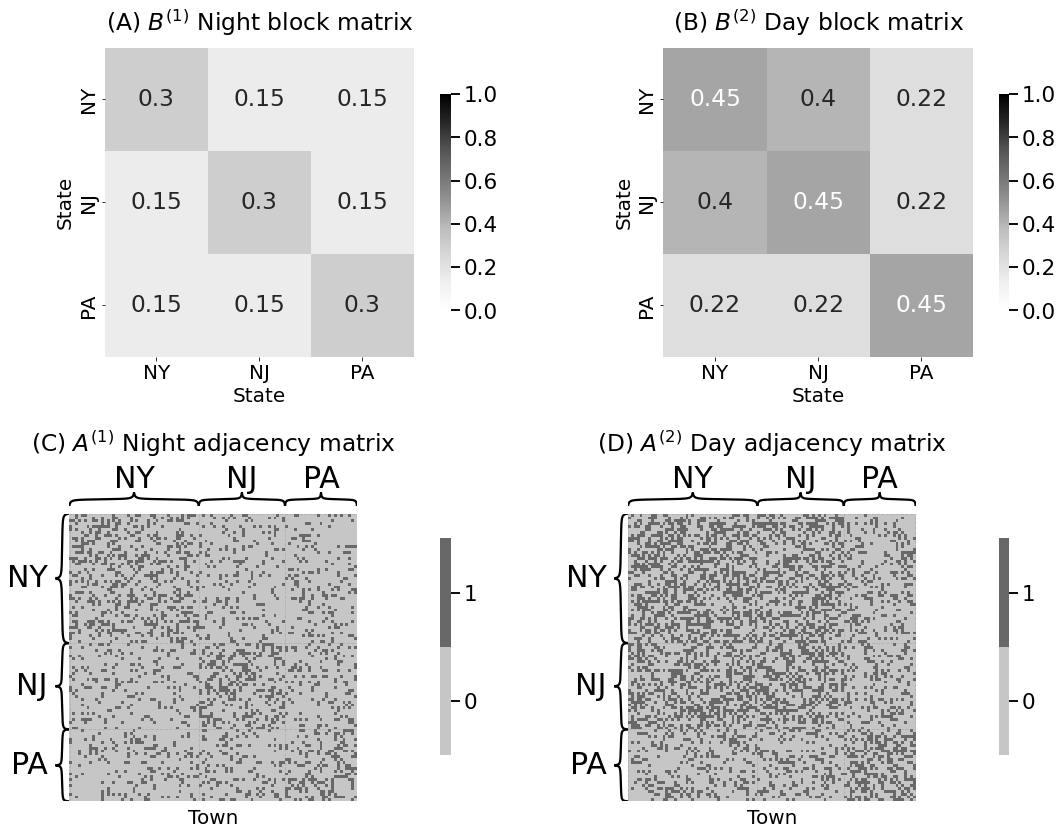
\includegraphics[width=\linewidth]{applications/ch8/Images/twosamp_sbm_ex.png}
    \caption[Two-sample SBM comparison]{\textbf{(A)} the block matrix for night time, \textbf{(B)} the block matrix for day time, \textbf{(C)} the adjacency matrix for night time, \textbf{(D)} the adjacency matrix for day time.}
    \label{fig:ch8:twosampsbm:ex}
\end{figure}

\subsection{Testing whether the block matrices in an SBM are different}

Based on what we learned above, we know ahead of time that the block matrices for the SBMs are different. However, how can we actually test this? Well, let's start by being clear about what we mean by "different". To make this a little big more mathemattical, we'll introduce some new variables for the block matrices during the day time ($B^{(1)}$) and at night time ($B^{(2)}$) clearly. The block matrices are:

\begin{align*}
    B^{(1)} &= \begin{bmatrix}
    b^{(1)}_{11} & b^{(1)}_{12} & b^{(1)}_{13} \\
    b^{(1)}_{21} & b^{(1)}_{22} & b^{(1)}_{23} \\
    b^{(1)}_{31} & b^{(1)}_{32} & b^{(1)}_{33}
    \end{bmatrix}; \;\;\; B^{(2)} = \begin{bmatrix}
    b^{(2)}_{11} & b^{(2)}_{12} & b^{(2)}_{13} \\
    b^{(2)}_{21} & b^{(2)}_{22} & b^{(2)}_{23} \\
    b^{(2)}_{31} & b^{(2)}_{32} & b^{(2)}_{33}
    \end{bmatrix}
\end{align*}
The hypothesis we want to test is the null hypothesis that the block matrices are the same, $H_0: B^{(1)} = B^{(2)}$, against the alternative hypothesis that the block matrices are different, $H_A: B^{(1)} \neq B^{(2)}$. For a matrix, remember that two matrices are equal if all of the entries are identical, and two matrices are unequal if at least one of the entries are unequal. We can reformulate the null and alternative hypotheses with this logic.

For the null hypothesis, $H_0: B^{(1)} = B^{(2)}$, the statement is therefore equivalent to saying that for all pairs of communities $k$ and $l$, $b^{(1)}_{kl} = b^{(2)}_{kl}$. We will write each of these statements down as individual hypotheses for all pairs of communities, using the convention $H_{0, kl}: b_{kl}^{(1)} = b^{(2)}_{kl}$. 

The null hypothesis $H_0$ is therefore equivalent to saying that for every pair of communities $k$ and $l$, $H_{0,kl}$ is true. 

For the alternative hypothesis, $H_A: B^{(1)} \neq B^{(2)}$, the statement is therefore equivalent to saying that for at least one pair of communities $k$ and $l$, $b^{(1)}_{kl} \neq b^{(2)}_{kl}$. We will write down each of these statements as well as individual hypotheses for all pairs of communities, using the convention $H_{A, kl} : b_{kl}^{(1)} \neq b^{(2)}_{kl}$. The alternative hypothesis $H_A$ is therefore equivalent to saying that for at least one pair of communities $k$ and $l$, that $H_{A,kl}$ is true.

Now that we have broken a statement about two matrices down into numerous statements about two probabilities, we have almost completed our job. As it turns out, we have already seen the way we will test this, back in testing for differences in Section \ref{sec:ch7:testing}. Seeking to test whether a pair of block probabilities between communities $k$ and $l$ are the same, $H_{0,kl}$, against whether the pair of block probabilities between communities $k$ and $l$ are different, $H_{A, kl}$, is the two-sample testing problem, like Section \ref{sec:ch7:testing:twosample}. We addressed this problem before using Fisher's exact test, and that is what we will do here, too.

Remember that with Fisher's exact test, for two probabilities that we want to compare, we construct a contingency table. In this case, we will have $\binom K 2 + K$ contingency tables (one for each unique pair of communities, plus the on-diagonal edges where both nodes have the same community), which are shown in Table \ref{tab:ch8:twosampl_sbm:cont}.

\begin{table}[h]
    \centering
    \begin{tabular}{c|c| c}
         & $(1)$, night time & $(2)$, day time  \\
         \hline
         Number of edges & $a$ & $b$ \\
         Number of non-edges &$c$ & $d$
    \end{tabular}
    \caption[Two-sample SBM contingency table.]{An example of a contingency table for testing for a difference in the block matrices between two SBMs. $\binom K 2$ of these contingency tables are constructed, corresponding to the contingency tables between nodes in community $k$ and $l$ for all possible pairs of communities.}
    \label{tab:ch8:twosampl_sbm:cont}
\end{table}

In the table, entry $a$ is the total number of edges between nodes of community $k$ with nodes of community $l$ in the daytime network, and $b$ is the total number of edges between nodes of community $k$ with nodes of community $l$ in the daytime network. The entry $c$ the total number of potential edges between nodes of community $k$ with nodes of community $l$ in the day time network that do not exist (the number of adjacencies with an adjacency of zero), and the entry $d$ is the total number of potential edges between nodes of community $k$ with nodes of community $l$ in the night time network that do not exist. 

We implement this using \texttt{numpy} and \texttt{scipy}, just like we did before, but this time for each pair of communities. To identify which adjacency matrix entries correspond to a given pair of communities, we use \texttt{np.outer}. Since the network is simple, we also exclude the on-diagonal entries, and avoid double counting by only looking at the upper-right triangle of the adjacency matrix:

\begin{lstlisting}[style=python]
from scipy.stats import fisher_exact

K = 3
Pvals = np.empty((K, K))
# fill matrix with NaNs
Pvals[:] = np.nan

# get the indices of the upper triangle of Aday
upper_tri_idx = np.triu_indices(Aday.shape[0], k=1)
# create a boolean array that is nxn
upper_tri_mask = np.zeros(Aday.shape, dtype=bool)
# set indices which correspond to the upper triangle to True
upper_tri_mask[upper_tri_idx] = True

for k in range(0, K):
    for l in range(k, K):
        comm_mask = np.outer(z == (k+1), z == (l + 1))
        table = [[Aday[comm_mask & upper_tri_mask].sum(), Anight[comm_mask & upper_tri_mask].sum()],
                 [(Aday[comm_mask & upper_tri_mask] == 0).sum(), (Anight[comm_mask & upper_tri_mask] == 0).sum()]]
        Pvals[k,l] = fisher_exact(table)[1]
\end{lstlisting}

This gives us a matrix of $p$-values, whose $p$-values correspond to tests of $H_{0, kl}$ against $H_{A, kl}$ for all pairs of communities $k$ and $l$. However, this still does not give us an answer to our original question, whether the block matrices $B^{(1)}$ and $B^{(2)}$ were the same against the alternative that the block matrices $B^{(1)}$ and $B^{(2)}$ were different.

\subsubsection*{Adjusting for multiple comparisons}

When performing multiple statistical tests, we run into the multiple hypothesis correction problem. Let’s imagine that we have $5000$ coins, and each of these coins has a true probability of landing on heads of $0.5$. We flip each coin 
$500$ times, and for each coin $i$, we estimate the probability that the coin lands on heads by just counting the number of heads and dividing by $500$. For each coin, we want to test whether the probability that the coin lands on heads is different from $0.5$. In symbols, we want to test $H_0^{(i)} : p^{(i)} = 0.5$ against $H_A^{(i)}: p^{(i)} \neq 0.5$. For this problem, an appropriate statistical test is known as the Binomial test, which is described in Appendix \ref{app:ch14:hypotest_intro}. For the purposes of this section, all that you need to know is that it is a way of testing whether the data supports (or does not support) that a probability is equal to a fixed constant. Let's run our experiments:

\begin{lstlisting}[style=python]
import numpy as np
from graspologic.simulations import er_np
import seaborn as sns
from scipy.stats import binom_test

ncoins = 5000 # the number of networks
p = 0.5  # the true probability
n = 500  # the number of flips

# the number of heads from each experiment
experiments = np.random.binomial(n, p, size=ncoins)

# perform binomial test to see if the number of heads we obtain supports that the
# true probabiily is 0.5
pvals = [binom_test(nheads_i, n, p=p) for nheads_i in experiments]
\end{lstlisting}


\begin{figure}
    \centering
    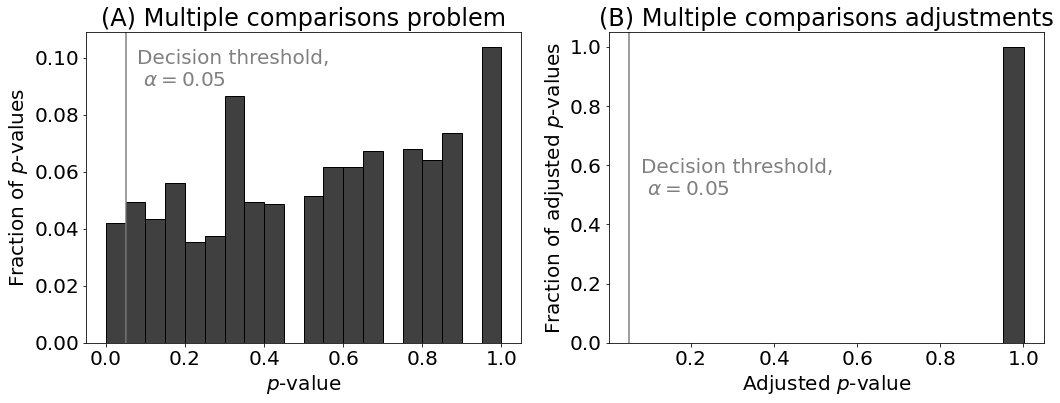
\includegraphics[width=\linewidth]{applications/ch8/Images/twosampsbm_mc.png}
    \caption{\textbf{(A)} a histogram of the $p$-values before multiple comparisons adjustment, \textbf{(B)} a histogram of the $p$-values after adjusting for multiple comparisons, by preserving the FWER via Holm-Bonferroni correction.}
    \label{fig:ch8:twosampsbm:mc}
\end{figure}
A histogram of the $p$-values from all $5000$ tests (one for each coin) are shown in Figure \ref{fig:ch8:twosampsbm:mc}(A). In general, we will correctly reject the alternative hypothesis, and accept the null hypothesis. This is great, since $p_i$ is, in fact, $0.5$ as specified by the null hypothesis $H_{0}^{(i)}$. However, we notice something particularly strange: For a portion of the tests, we are, in-fact, wrong. We obtain many $p$-values which are under our decision threshold of $\alpha = 0.05$, and would incorrectly report that the alternative hypothesis is correct, and $p_i$ is not $0.5$. This is wrong, and extremely problematic! Remember that the $p$-value was defined as the probability that the null hypothesis (here, that $p_i = 0.5$) would be incorrectly rejected in favor of the alternative hypothesis (here, that $p_i \neq 0.5$). In fact, if the null hypothesis were true, we would expect to see $p$-values of at most $\alpha$ being reported about $\alpha$ of the time (this assumes all of the coins are independent, but even when they are not all independent, we still obtain a similarly shocking conclusion). This means that with $n=5000$ tests and $\alpha = 0.05$, we would expect to be wrong about $n\cdot \alpha = 50$ times.

Basically, the problem here is that while each test individually only has a $\alpha = 0.05$ chance of incorrectly rejecting the null hypothesis (when it is true), by running multiple tests, we have increased the familywise error rate to be well north of $\alpha = 0.05$. The \textit{familywise error rate} (FWER) is the probability that we made an error and incorrectly rejected the null hypothesis for any one of the hypothesis tests we ran. You can read more about this problem here \cite{Ryan1959Jan}.

As practicians, it feels like it would be pretty problematic to report an analysis and know that an arbitrary fraction of your conclusions are wrong just by random chance. For this reason, a focus of statistics in recent decades has been the development of methods which, in effect, inflate the $p$-values based on the number of tests that we perform, so that we run into this issue at much lower rate than $\alpha$ of the time. These strategies are collectively known as \textit{multiple comparisons adjustments}. We won't go into too many details with how multiple comparisons adjustments are performed, but in general given a list of $p$-values \texttt{pvals}, you can adjust the $p$-values using the \texttt{multipletests()} method from \texttt{statsmodels}. This will give you protection for this ``multiple comparisons'' issue in your analyses, and make you a more conservative statistician. Like in Section \ref{sec:ch8:twosample:lpt_vs_ldt}, conservative statistical approaches are approaches which tend to err on the side of caution.

Let's see what happens when we adjust our $p$-values here using a popular method called Bonferroni-Holm adjustment \cite{Holm1979}:
\begin{lstlisting}[style=python]
from statsmodels.stats.multitest import multipletests

alpha = 0.05  # the desired alpha of the test
_, adj_pvals, _, _ = multipletests(pvals, alpha=alpha, method="holm")
\end{lstlisting}

A histogram of the $p$-values after adjustment is shown in Figure \ref{fig:ch8:twosampsbm:mc}(B). After adjusting for multiple comparisons, we end up with all of the $p$-values being $1$. Therefore, we never incorrectly reject the null hypothesis anymore.

In general, for multiple hypothesis correction, we recommend using Holm-Bonferroni correction, which is encoded with the parameter \texttt{method="holm"}. We recommend the use of the Holm-Bonferroni approach because it ensures that our $p$-value produced by using multiple statistical tests controls the FWER with no requirements as to the problem we glossed over previously, the dependence of the hypotheses being tested. This may give us adjusted $p$-values that are a little higher than several other methods (such as the popular Benjamini-Hochberg procedure), but in general we prefer to err on the side of caution when reporting scientific discoveries and do not want to spend effort investigating hypothetical dependencies amongst our hypothesis tests.

Let's adjust the $p$-values that we estimated for the pairwise community comparisons for our networks, upper-right symmetrize the resulting matrix of $p$-values (because we only ran tests on the upper-right triangle of the adjacency matrix), and then plot the result:
\begin{lstlisting}[style=python]
from graspologic.utils import symmetrize

Pvals_adj = multipletests(Pvals.flatten(), method="holm")[1].reshape(K, K)
Pvals_adj = symmetrize(Pvals_adj, method="triu")
\end{lstlisting}

\begin{figure}
    \centering
    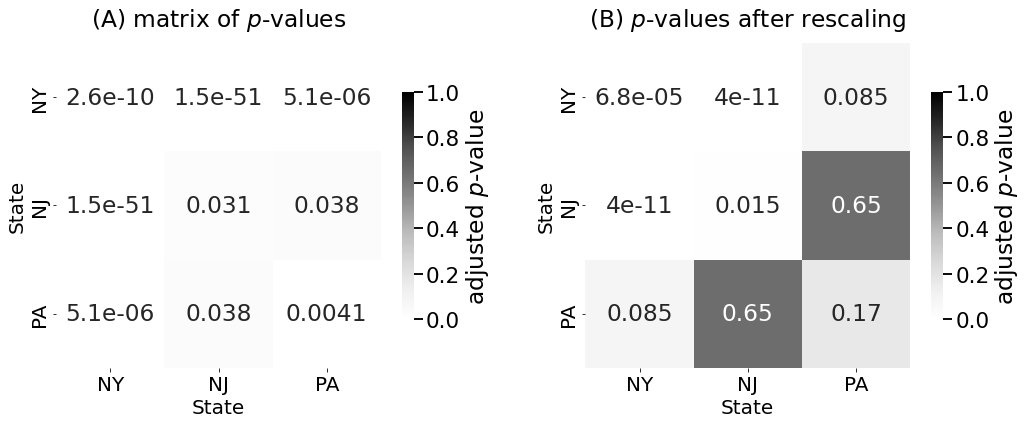
\includegraphics[width=\linewidth]{applications/ch8/Images/twosamp_sbm_pvals.png}
    \caption[$p$-values for differences between block matrices]{\textbf{(A)} $p$-values for test of a difference between the block matrices, \textbf{(B)} $p$-values for test of a difference between the block matrices, after rescaling.}
    \label{fig:ch8:twosampsbm:pval_mtx}
\end{figure}

The matrix of $p$-values (after adjustment for multiple comparisons) is shown in Figure \ref{fig:ch8:twosampsbm:pval_mtx}(A). The $p$-values are all extremely small, so we can conclude that the block matrices $B^{(1)}$ and $B^{(2)}$ differ for all entries. The $p$-value for the test of $H_0$ that the block matrices are identical against $H_A$ that the block matrices are different can be taken to be the minimum of all of the adjusted $p$-values:

\begin{lstlisting}[style=python]
pval_dif = Pvals_adj.min()
print("p-value of block matrix difference: {:.4f}".format(pval_dif))
# p-value of block matrix difference: 0.0000
\end{lstlisting}
which is so small that it rounds to $0$. With $\alpha = 0.05$ as usual, we reject the null hypothesis that the block matrices are identical in favor of the alternative that the block matrices are different. 

\subsection{Testing whether the block matrices in an SBM are multiples of one another}

Back in Section \ref{sec:ch5:prop:rndeg} we learned about a useful summary statistic for random networks, known as the expected density. The expected network density could be written as:
\begin{align*}
\mathbb E[density(\mathbf A)] &= \frac{\sum_{i = 1}^n \mathbb E[\mathbf d_i]}{n(n - 1)} 
\end{align*}
Which could be thought of as the expected average degree of each node in the network, divided by the maximum possible degree each node could have. 

As it turns out, the network density plays an extremely large role in virtually every property of networks which we estimate in machine learning, including the block matrices. Remember from Concept \ref{box:ch5:dcsbm:exp_deg}, that for a $SBM_n(\vec z, B)$ random network, the average degree for a node in community $k$ was:
\begin{align*}
    \mathbb E[\mathbf d_i ; z_i = k] &= \sum_{l \neq k} n_l b_{lk} + (n_k - 1)b_{kk}
\end{align*}
so it is clear that the expected node degree is a function of the block matrix. As the expected density is a function of the expected degrees, the expected density is a function of the block matrix, too. We could also reverse this argument, and establish a relationship between the block matrices and the expected density in the network.

This means that if the expected densities are different, the block matrices will, by default, also be different.

For instance, in our example, we know that the probability of an edge existing between two cities is, in general, about $50\%$ higher during the daytime compared to the night time. We don't want to have our answer just be a product of the fact that there were just more edges in the daytime network. Rather, we want to find the topological difference between the two networks; that is, that the day time driving patterns between New Jersey and New York towns went above and beyond the $50\%$ increase we otherwise saw. For this reason, we revamp our hypothesis a little bit.

If you remember, our hypothesis that we ran above was the null hypothesis $H_0: B^{(1)} = B^{(2)}$ that the two block matrices are the same against the alternative $H_A: B^{(1)} \neq B^{(2)}$ that the block matrices differ. We will change this up a little bit. Now, our null hypothesis becomes $H_0: B^{(1)} = \alpha\cdot B^{(2)}$ that the two block matrices are the same up to a rescaling against $H_A: B^{(2)} \neq \alpha\cdot B^{(2)}$, that they differ even after possible rescalings. How do we interpret this?

In this case, the value $\alpha$ is chosen to be the difference in the expected network densities between the day time and night time networks, the quantity $\alpha = \frac{p^{(1)}}{p^{(2)}}$. In practice, what we use is an estimate of this quantity, $\hat \alpha = \frac{\hat p^{(1)}}{\hat p^{(2)}}$, where $\hat p^{(1)}$ is the network density of the night time network and $\hat p^{(2)}$ is the network density of the day time network. Accepting the alternative hypothesis here means that the block matrices of the day and night time network are not simply multiples of each other.

\begin{floatingbox}[h]\caption{Case Study: Bilateral symmetry in fruit fly brains}
\label{box:ch8:twosamp_sbm:conn}
It is fairly well-established that the brain of human beings is asymmetric: different sides of your brain are responsible for related, but distinct, functions \cite{Springer2001Sep}. This was definitively established in the 1860s by a scientist named Paul Broca, who discovered that patients with brain lesions to the same area of the left frontal portion of the brain experienced similar symptoms of speech loss. That two patients with similar lesions experienced the same symptoms provided evidence that brain function was \textit{localized}, in that different areas of the brain were responsible for different functions. Related observations made by psychologists led to conclusions that took this a step further, that different hemispheres of the brain were responsible for different functions.

In a recent paper \cite{Pedigo2022Nov}, investigators were able to connect a similar ``localization of connectivity'' in the wiring of the brain itself. The investigators used connectomes of a fruit fly for the left and right hemispheres, where the nodes were individual neurons and the edges were individual connections (called \textit{synapses}) between these neurons. Using the methods that we explained above, they were able to show that some types of cells in the brain had totally different densities of edges between the two hemispheres. After accounting for these hemisphere density disparities, several different cell types had similar connectivity patterns.
\end{floatingbox}

We address this problem very similarly to above, instead using the chi-squared test for non-unity probability ratios from \cite{Dunnett1977Dec, Chan2003Jan, Miettinen1985Apr}. We covered the chi-squared test in Section \ref{sec:ch7:modelselect} when we were covering model selection. We implement this using the bilateral connectome package \cite{neurodata2023Feb}, again showing the $p$-value matrix to visualize which combinations of communities are substantially different. This approach is described in \cite{Pedigo2022Nov}:

\begin{lstlisting}[style=python]
from pkg.stats import stochastic_block_test, combine_pvalues

stat, _, misc = stochastic_block_test(Anight, Aday,
    labels1=z, labels2=z, density_adjustment=True)
Pval_adj_rescaled = np.array(misc["corrected_pvalues"])
\end{lstlisting}

This new matrix of $p$-values is shown in Figure \ref{fig:ch8:twosampsbm:pval_mtx}(B), This shows that after we adjust the block matrix for changes in network density, the difference in the block probability for traveling between New York and New Jersey is still significant. This means that the density-adjusted block matrices are different, since the minimum corrected $p$-value is less than $0.05$.


The interpretation here is that, after adjusting for density, we can still reject the null hypothesis in favor of the alternative that the block matrices for day and night time are different, and that this difference can be accounted for by different traffic patterns between New York and New Jersey in day time versus night time. For an example of the use of these strategies in practice, check out Case Study \ref{box:ch8:twosamp_sbm:conn}.


\newpage


\section{The graph matching problem}
\label{sec:ch8:gm}

\bibliographystyle{vancouver}
\bibliography{references}